\documentclass[a4paper,french]{paper}
\usepackage{../../_latex_assets/villemejane_iogs_ceti}

%Informations about this document 
%------------------------------------------
\def\module{Ingénierie Electronique pour le Traitement de l'Information}
\def\moduleAbrege{6N-047-SCI / IéTI}
\def\annee{}

\def\titre{TD 2 / Pilotage d'une source à diodes}
\author{Julien VILLEMEJANE}

\subtitle{TD 2}
\institution{LEnsE / Institut d'Optique Graduate School}

\title{\titre}
\begin{document} 
%Beginning First Page. 
%------------------------------------------
\enteteThematiqueObligatoire{}

%Beginning Content. 
%------------------------------------------
\vspace{-1cm}
%%%%%%%%%%%%%%%%%%%
\subsection*{Transistors bipolaires}

Les transistors bipolaires sont des composants amplificateurs de courant à 3 broches : l'émetteur, le collecteur et la base.

\begin{center}
	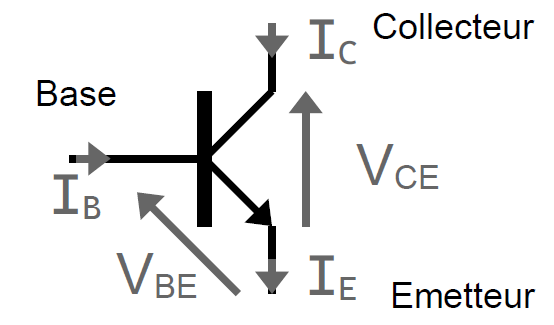
\includegraphics[width=5cm]{images/bipolaire.png}
\end{center}

Les différents courants et tensions sont régis par les relations suivantes :

$$I_C = \beta \cdot I_B \qquad et \qquad I_E = I_C + I_B$$

$$I_C = \beta \cdot I_{BS} \cdot \exp(V_{BE}/U_T)$$

où $U_T$, $I_{BS}$ et $\beta$ sont des paramètres intrinsèques du transistor.


%%%%%%%%%%%%%%%%%%%

\encadreTDExo{1 - Miroir de courant}{
On s'intéresse au montage suivant :

\begin{center}
	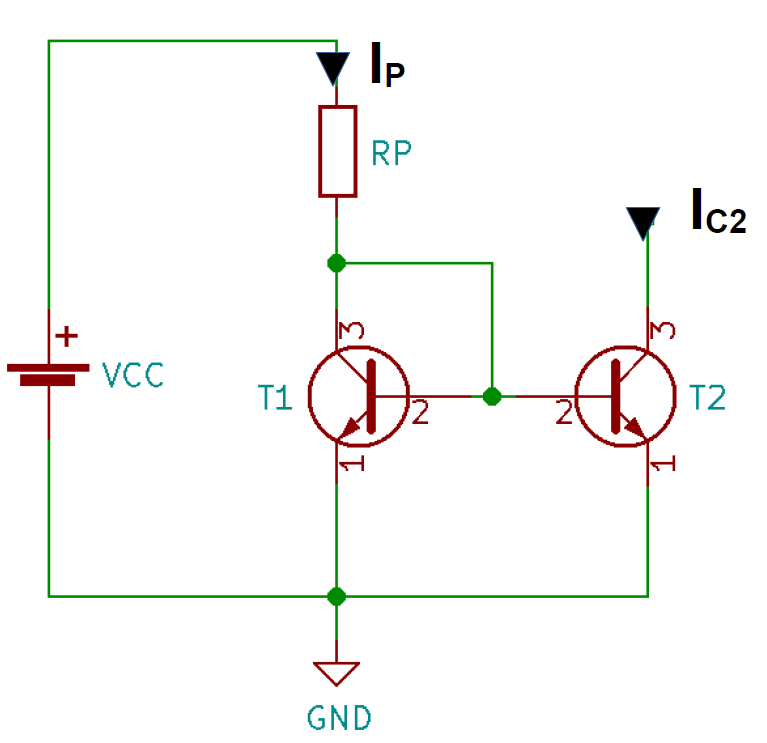
\includegraphics[width=7cm]{images/mirroir_courant_1.png}
\end{center}


\begin{enumerate}
	\item Calculez $I_{C2}$ en fonction de $I_P$.
	\item Calculez la puissance dissipée par la résistance $R_P$
	\item Retrouve-t-on cette structure dans le composant AL5809 (dont une partie de la documentation est fournie en annexe) ?
	\item Expliquez le fonctionnement de ce composant. Quel est l'intérêt du montage de la figure 3 (p.5 de la documentation) par rapport à celui de la figure 2 ?
\end{enumerate}
}

%------------------------------------------
%%%%%%%%%%%%%%%%%%%
\encadreTDExo{2 - Driver de LEDs}{
On donne le schéma interne du composant NCR320U :

\begin{center}
	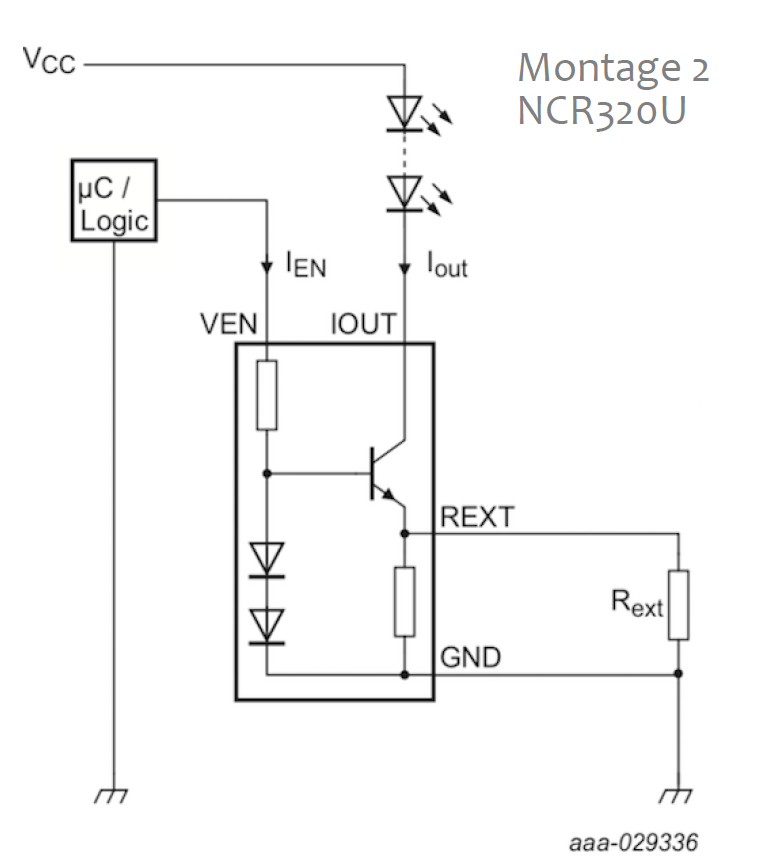
\includegraphics[width=10cm]{images/mirroir_courant_2.png}
\end{center}

\begin{enumerate}
	\item Calculez le courant $I_{out}$ en fonction de $R_{ext}$ et précisez le rôle de cette résistance.
	\item Calculez le courant $I_{en}$ en fonction de $V_{en}$ et précisez le rôle de cette tension.
	\item Expliquez le rôle de ce composant et son fonctionnement.
\end{enumerate}
}


%%%%%%%%%%%%%%%%%%%
\encadreTDExo{3 - Miroir bis}{
Soit le circuit suivant :

\begin{center}
	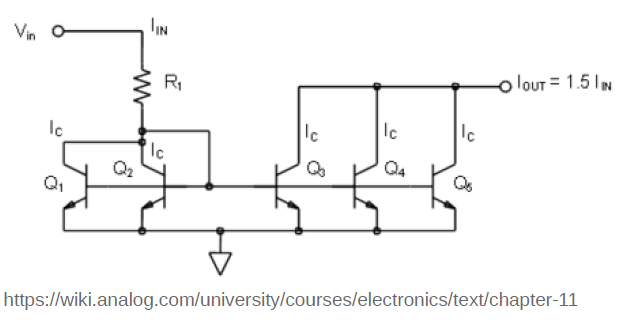
\includegraphics[width=10cm]{images/mirroir_courant_3.png}
\end{center}

Expliquez le fonctionnement et l'intérêt de ce montage.
}



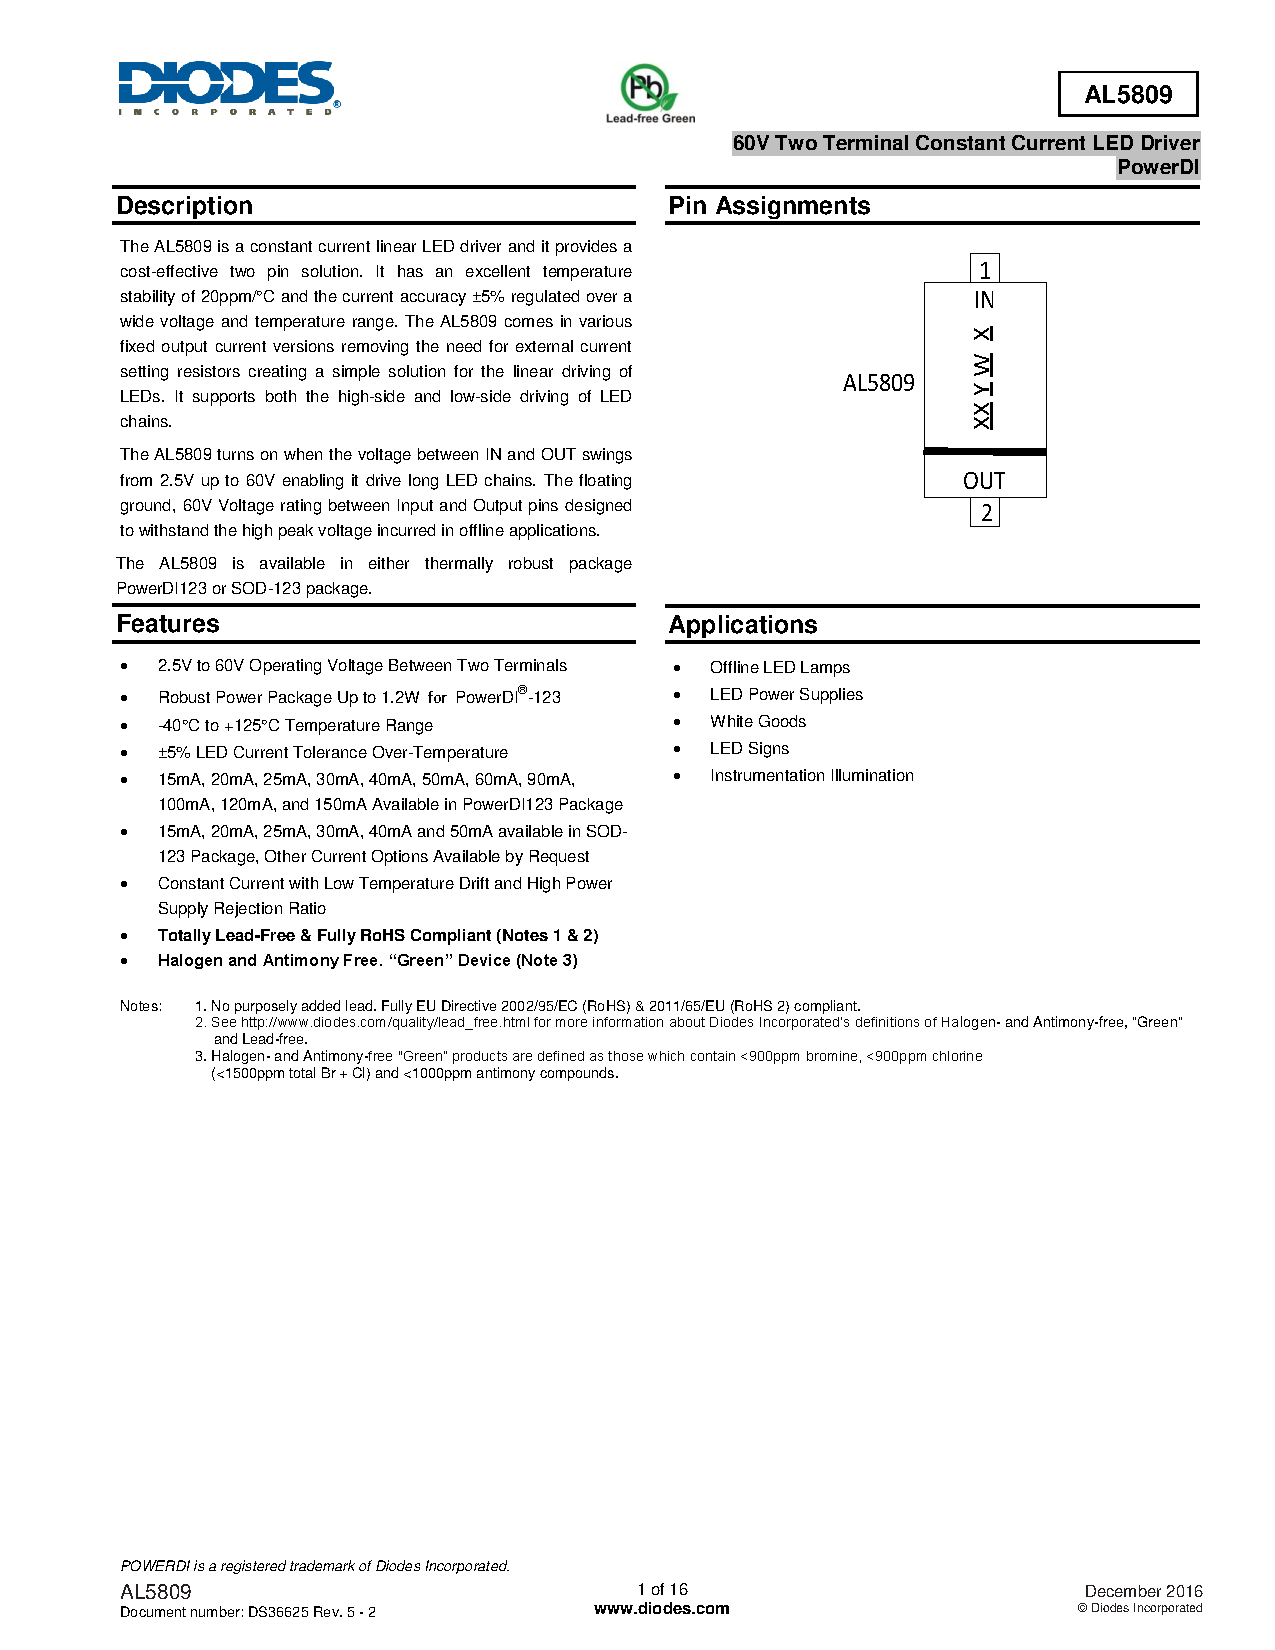
\includepdf[pages={1-2,4-5}]{docs/AL5809.pdf}

\end {document}